\documentclass[a4paper,11pt]{extarticle}

\usepackage[utf8]{inputenc} %кодировка
\usepackage[T1,T2A]{fontenc} % тоже кодировка
\usepackage[english,russian]{babel} %языки

\usepackage{multirow}
\usepackage{tabularx,booktabs}
\usepackage{floatrow}


\usepackage{graphicx, float} %пакет для единого оформления всех плавающих объектов (избегаем повторяющихся команд в документе)

\DeclareGraphicsExtensions{.pdf,.png,.jpg,.eps}%форматы
\usepackage{titlesec}
\setcounter{secnumdepth}{4}
\titleformat{\paragraph}
{\normalfont\normalsize\bfseries}{\theparagraph}{1em}{}
\titlespacing*{\paragraph}
{0pt}{3.25ex plus 1ex minus .2ex}{1.5ex plus .2ex}

\graphicspath{{images/}} % выбираем папку, в которую сохраняем все рисунки, чтобы не было хаоса файлов

\usepackage{amsmath,amssymb}%математические формулы и символы

\usepackage[a4paper,left=30mm,right=15mm,top=20mm,bottom=20mm]{geometry} % устанавливает поля документа

\parindent=4ex %красная строка
\parskip=5mm %расстояние между параграфами
\usepackage{indentfirst} %делать отступ в начале параграфа

\usepackage{hyperref} % добавление ссылок

\def\hmath$#1${\texorpdfstring{{\rmfamily\textit{#1}}}{#1}}
%настройка подписей плавающих объектов

\makeindex %нумерация

\usepackage{array,graphicx,caption} %картинки, подписи, таблицы
%\usepackage{endfloat} - для вывода картинок со списком в конце файла

\usepackage{caption} %подписи к картинкам

\usepackage[labelformat=simple]{subcaption} %для subfigure
\renewcommand\thesubfigure{(\alph{subfigure})}

\usepackage[export]{adjustbox} %чтобы влево-вправо картинки ставить

\usepackage[labelformat=simple]{subcaption}
% метка subfigure: "(а)" вместо дефолтного "а"

\renewcommand\thesubfigure{(\alph{subfigure})} % для продвинутого captionof

\usepackage{afterpage,placeins} % для барьеров

\usepackage{wrapfig} %добавление wrapfig

\usepackage[nottoc]{tocbibind} %подключает в содержание список лит-ры

\usepackage{multicol}

\usepackage{listings}

\usepackage[normalem]{ulem}
\usepackage{verbatim}
\usepackage[russian]{babel}

\usepackage{xcolor}

%New colors defined below
\definecolor{codegreen}{rgb}{0,0.6,0}
\definecolor{codegray}{rgb}{0.5,0.5,0.5}
\definecolor{codepurple}{rgb}{0.58,0,0.82}
\definecolor{backcolour}{rgb}{0.95,0.95,0.92}

%Code listing style named "mystyle"
\lstdefinestyle{mystyle}{
  backgroundcolor=\color{backcolour}, commentstyle=\color{codegreen},
  keywordstyle=\color{magenta},
  numberstyle=\tiny\color{codegray},
  stringstyle=\color{codepurple},
  basicstyle=\ttfamily\footnotesize,
  breakatwhitespace=false,
  breaklines=true,
  captionpos=b,
  keepspaces=true,
  numbers=left,
  numbersep=5pt,
  showspaces=false,
  showstringspaces=false,
  showtabs=false,
  tabsize=2
}

%"mystyle" code listing set
\lstset{style=mystyle}


\begin{document}

\begin{center}
МИНИСТЕРСТВО НАУКИ И ВЫСШЕГО ОБРАЗОВАНИЯ РОССИЙСКОЙ ФЕДЕРАЦИИ\\
\hfill \break
ФЕДЕРАЛЬНОЕ ГОСУДАРСТВЕННОЕ АВТОНОМНОЕ \\ ОБРАЗОВАТЕЛЬНОЕ УЧРЕЖДЕНИЕ ВЫСШЕГО ОБРАЗОВАНИЯ \\
“МОСКОВСКИЙ ФИЗИКО-ТЕХНИЧЕСКИЙ ИНСТИТУТ (НАЦИОНАЛЬНЫЙ ИССЛЕДОВАТЕЛЬСКИЙ УНИВЕРСИТЕТ)” \\

\hfill \break
Физтех-школа радиотехники и компьютерных технологий\\
\vspace{2.5cm}
\large{\textbf{Отчёт по лабораторной работе № 2.1.4}}\\
\large{\textbf{"Определение теплоемкости твердых тел"}}\\
\hfill \break
\end{center}

\vspace{5cm}

\begin{flushright}
Выполнил:\\
Студент гр. Б01-305\\
Миннахметов Артур\\
\end{flushright}

\vfill


\begin{center} Долгопрудный, 2024 \end{center}

\thispagestyle{empty}
\newpage


\textbf{Цель работы: }
исследование резонанса токов в параллельном колебательном контуре с изменяемой ёмкостью, получение амплитудно-частотных и фазово-частотных характеристик, определение основных параметров контура.
	\n\n
	\textbf{В работе используются: }
	генератор сигналов произвольной формы, цифровой осциллограф с функцией быстрого преобразования Фурье.

%
%\subsection*{Разложение сложных сигналов на периодические колебания}
%В работе используется разложение в сумму синусов и косинусов с различными аргументами или, как чаще его называют, \textit{разложение в ряд Фурье}.
%\n\n
%Пусть задана функция $f(t)$, которая периодически повторяется с частотой $\Omega_1 = \dfrac{2\pi}{T}$, где $T$ --- период повторения импульсов. Её разложение в ряд Фурье имеет вид
%\begin{equation}
%f(t) = \dfrac{a_0}{2} + \sum\limits_{n = 1}^{\infty}\left[a_n \cos \left(n \Omega_1t\right) + b_n \sin \left(n \Omega_1t\right)\right],
%\end{equation}
%\begin{equation}
%f(t) = \dfrac{a_0}{2} + \sum\limits_{n = 1}^{\infty}A_n \cos \left(n\Omega_1t-\psi_n\right).
%\end{equation}
%Если сигнал чётен относительно $t=0$, в тригонометрической записи остаются только члены с косинусами. Для нечетной - наоборот.
%\n\n
%Коэффициенты определяются по формуле:
%\begin{equation}
%\begin{array}{c}
%a_n  = \dfrac{2}{T}\int\limits_{t_1}^{t_1+T}f(t)\cos\left(n \Omega_1 t\right) dt, \ \ \
%b_n = \dfrac{2}{T}\int\limits_{t_1}^{t_1+T}f(t)\sin\left(n \Omega_1 t\right) dt.
%\end{array}
%\end{equation}
%\n
%Здесь $t_1$ --- время, с которого мы начинаем отсчет.
%\n\n
%Сравнив формулы $(1)$ и $(2)$, можно получить выражения для $A_n$  и $\psi_n$:
%\begin{center}
%    $A_n = \sqrt{a_n^2+b_n^2}, \ \ \
%    \psi_n = \arctg \dfrac{b_n}{a_n}.$
%\end{center}
%\subsection*{Периодическая последовательность прямоугольных импульсов}
%\begin{center}
%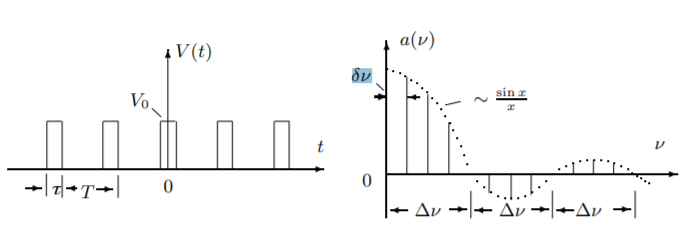
\includegraphics[scale=0.9]{pic1.png}
%\end{center}
%Введем величину: $\Omega_1 = \dfrac{2\pi}{T}$,
%где $T$ --- период повторения импульсов.
%\n\n
%Коэффициенты при косинусных составляющих будут равны
%\begin{center}
%    $a_n = \dfrac{2}{T}\int\limits_{-\tau/2}^{\tau/2}V_0\cos\left(n\Omega_1 t\right)dt = 2V_0\dfrac{\tau}{T}\dfrac{\sin\left(n\Omega_1\tau/2\right)}{n\Omega_1\tau/2} \sim \dfrac{\sin x}{x}.$
%\end{center}
%\n
%Здесь $V_0$ - амплитуда сигнала. Поскольку наша функция четная, то $b_n = 0$. Пусть $T$ кратно $\tau$. Тогда введем ширину спектра, равную $\Delta \omega$ --- расстояние от главного максимума до первого нуля огибающей, возникающего, как нетрудно убедиться при $n = \dfrac{2\pi}{\tau \Omega_1}$. При
%этом
%\begin{center}
%    $\Delta \omega \tau \simeq 2\pi \Rightarrow \Delta \nu \Delta t \simeq 1.$
%\end{center}
%\subsection*{Периодическая последовательность цугов}
%\begin{center}
%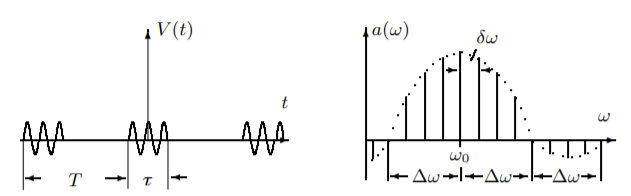
\includegraphics[scale=0.9]{pic2.png}
%\end{center}
%Возьмём цуги колебания $V_0 \cos(\omega_0 t)$ с длительностью цуга $\tau$ и периодом повторений $T$.\n\n
%Функция $f(t)$ снова является четной относительно $t = 0$. Коэффициент при $n$-ой гармонике согласно формуле $(3)$ равен
%\begin{center}
%    $a_n = \dfrac{2}{T}\int\limits_{-\tau/2}^{\tau/2}V_0 \cos \left(\omega_0t\right) \cdot \cos\left(n \Omega_1t\right)dt = V_0 \dfrac{\tau}{T}\left( \dfrac{\sin\left[\left(\omega_0 - n \Omega_1\right)\dfrac{\tau}{2}\right]}{\left( \omega_0 - n \Omega_1\right) \dfrac{\tau}{2}} + \dfrac{\sin\left[\left(\omega_0 + n \Omega_1\right)\dfrac{\tau}{2}\right]}{\left( \omega_0 + n \Omega_1\right) \dfrac{\tau}{2}}\right).$
%\end{center}
%Пусть $T$ кратно $\tau$. Тогда спектры последовательности прямоугильных сигналов и цугов аналогичны, но максимумы сдвинуты на $\omega_0$.
%\subsection*{Амплитудно-модулированные колебания}
%\begin{center}
%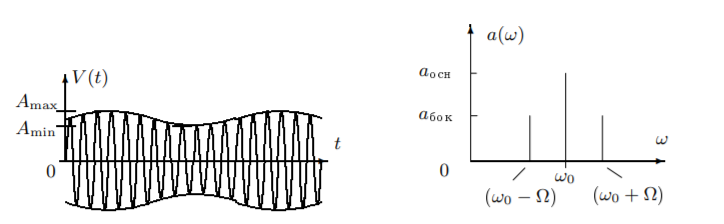
\includegraphics[scale=0.9]{pic3.png}
%\end{center}
%Рассмотрим гармонические колебания высокой частоты $\omega_0$, амплитуда которых медленно меняется по гармоническому закону с частотой $\Omega \ll \omega_0$:
%\begin{center}
%    $f(t) = A_0 \left[1+m\cos \Omega t\right] \cos \omega_0 t.$
%\end{center}
%Коэффициент $m$ называется \textit{глубиной модуляции}. При $m < 1$ амплитуда меняется от минимальной $A_{min} = A_0(1-m)$ до максимальной $A_{max} = A_0(1+m)$. Глубина модуляции может быть представлена в виде
%\begin{equation}
%m = \dfrac{A_{max}-A_{min}}{A_{max}+A_{min}}.
%\end{equation}
%Простым тригонометрическим преобразованием уравнения $(4)$ можно найти спектр колебаний:
%\begin{center}
%    $f(t) = A_0 \cos \omega_0t + \dfrac{A_0m}{2} \cos \left(\omega_0 + \Omega\right)t + \dfrac{A_0m}{2}\cos\left(\omega_0 - \Omega\right)t.$
%\end{center}

\section*{Теоретические сведения}

\subsection*{Разложение сложных сигналов на периодические колебания}
В работе используется разложение функции в сумму синусов и косинусов с различными аргументами или, как чаще его называют, \textit{разложение в ряд Фурье}.
\n\n
Пусть задана функция $f(t)$, которая периодически повторяется с частотой $\Omega_1 = \dfrac{2\pi}{T}$, где $T$ --- период повторения импульсов. Её разложение в ряд Фурье имеет вид:
\begin{equation}
f(t) = \dfrac{a_0}{2} + \sum\limits_{n = 1}^{\infty}\left[a_n \cos \left(n \Omega_1t\right) + b_n \sin \left(n \Omega_1t\right)\right]
\end{equation}
или
\begin{equation}
f(t) = \dfrac{a_0}{2} + \sum\limits_{n = 1}^{\infty}A_n \cos \left(n\Omega_1t-\psi_n\right).
\end{equation}
Если сигнал чётен относительно $t=0$, в тригонометрической записи остаются только члены с косинусами. Для нечетного - наоборот.
\n\n
Коэффициенты определяются по формулам:
\begin{equation}
\begin{array}{c}
a_n  = \dfrac{2}{T}\int\limits_{t_1}^{t_1+T}f(t)\cos\left(n \Omega_1 t\right) dt,\\
\\
b_n = \dfrac{2}{T}\int\limits_{t_1}^{t_1+T}f(t)\sin\left(n \Omega_1 t\right) dt.
\end{array}
\end{equation}
Здесь $t_1$ --- время, с которого мы начинаем отсчет.
\n\n
Сравнив формулы $(1)$ и $(2)$, можно получить выражения для $A_n$  и $\psi_n$:
\begin{equation}
\begin{array}{l}
A_n = \sqrt{a_n^2+b_n^2},\\
 \psi_n = \arctan \dfrac{b_n}{a_n}.
\end{array}
\end{equation}
\subsection*{Периодическая последовательность прямоугольных импульсов}
\begin{center}
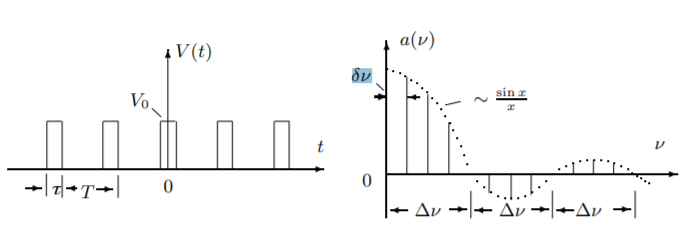
\includegraphics[scale=0.9]{2.png}
\end{center}
Введем величину: $\Omega_1 = \dfrac{2\pi}{T}$,
где $T$ --- период повторения импульсов.
\n\n
Коэффициенты при косинусных составляющих будут равны:
\begin{equation}
a_n = \dfrac{2}{T}\int\limits_{-\tau/2}^{\tau/2}V_0\cos\left(n\Omega_1 t\right)dt = 2V_0\dfrac{\tau}{T}\dfrac{\sin\left(n\Omega_1\tau/2\right)}{n\Omega_1\tau/2} \sim \dfrac{\sin x}{x}.
\end{equation}
\n
Здесь $V_0$ - амплитуда сигнала.
\n
Поскольку наша функция четная, $b_n = 0$.
\n
Пусть $T$ кратно $\tau$. Тогда введем ширину спектра, равную $\Delta \omega$ --- расстоянию от главного максимума до первого нуля огибающей, возникающего, как нетрудно убедиться, при $n = \dfrac{2\pi}{\tau \Omega_1}$. При
этом:
\begin{equation}
\Delta \omega \tau \simeq 2\pi \Rightarrow \Delta \nu \Delta t \simeq 1.
\end{equation}
\n В работе мы будем проверять справедливость этой формулы.
\subsection*{Периодическая последовательность цугов}
\begin{center}
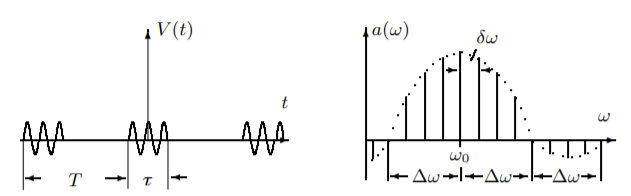
\includegraphics[scale=0.9]{3.png}
\end{center}
Возьмём цуги колебания $V_0 \cos(\omega_0 t)$ с длительностью цуга $\tau$ и периодом повторений $T$.\n\n
Функция $f(t)$ снова является четной относительно $t = 0$. Коэффициент при $n$-ой гармонике согласно формуле $(3)$ равен:
\begin{equation}
a_n = \dfrac{2}{T}\int\limits_{-\tau/2}^{\tau/2}V_0 \cos \left(\omega_0t\right) \cdot \cos\left(n \Omega_1t\right)dt = V_0 \dfrac{\tau}{T}\left( \dfrac{\sin\left[\left(\omega_0 - n \Omega_1\right)\dfrac{\tau}{2}\right]}{\left( \omega_0 - n \Omega_1\right) \dfrac{\tau}{2}} + \dfrac{\sin\left[\left(\omega_0 + n \Omega_1\right)\dfrac{\tau}{2}\right]}{\left( \omega_0 + n \Omega_1\right) \dfrac{\tau}{2}}\right).
\end{equation}
Пусть $T$ кратно $\tau$. Тогда спектры последовательности прямоугольных сигналов и цугов аналогичны, но максимумы сдвинуты на $\omega_0$.
\subsection*{Амплитудно-модулированные колебания}
\begin{center}
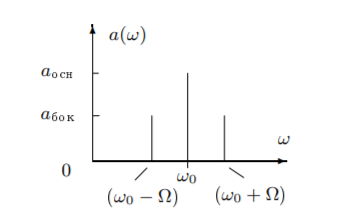
\includegraphics[scale=0.9]{4.png}
\end{center}
Рассмотрим гармонические колебания высокой частоты $\omega_0$, амплитуда которых медленно меняется по гармоническому закону с частотой $\Omega \ll \omega_0$:
\begin{equation}
f(t) = A_0 \left[1+m\cos \Omega t\right] \cos \omega_0 t.
\end{equation}
Коэффициент $m$ называется \textit{глубиной модуляции}. При $m < 1$ амплитуда меняется от минимальной $A_{min} = A_0(1-m)$ до максимальной $A_{max} = A_0(1+m)$. Глубина модуляции может быть представлена в виде
\begin{equation}
m = \dfrac{A_{max}-A_{min}}{A_{max}+A_{min}}.
\end{equation}
Простым тригонометрическим преобразованием уравнения $(8)$ можно найти спектр колебаний:
\begin{equation}
f(t) = A_0 \cos \omega_0t + \dfrac{A_0m}{2} \cos \left(\omega_0 + \Omega\right)t + \dfrac{A_0m}{2}\cos\left(\omega_0 - \Omega\right)t.
\end{equation}
\n
В дальнейшем мы будем использовать эту формулу.

\section*{Результаты измерений}

\subsection*{Исследование спектра периодических последовательностей прямоугольных импульсов}
Устанавив прямоугольные колебания c $\nu_{\text{повт}} = 1$ кГц (период $T = 1$ мс) и длительностью импульса $\tau = T/20 = 50$ мкс, мы получили на экране спектр сигнала и, изменяя либо $\tau$, либо $\nu_{\text{повт}}$, наблюдали, как изменяется спектр.
\begin{figure}[H]
    \centering
    \subfloat[$\nu_{\text{повт}} = 1$ кГц, $\tau = 50$ мкс]{{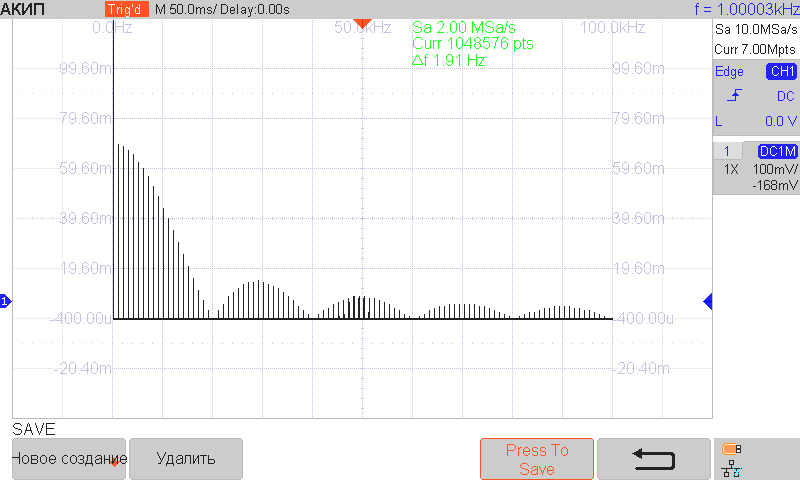
\includegraphics[width=0.5\textwidth]{AKIP0001.png}}}
    \subfloat[$\nu_{\text{повт}} = 1.5$ кГц, $\tau = 50$ мкс]{{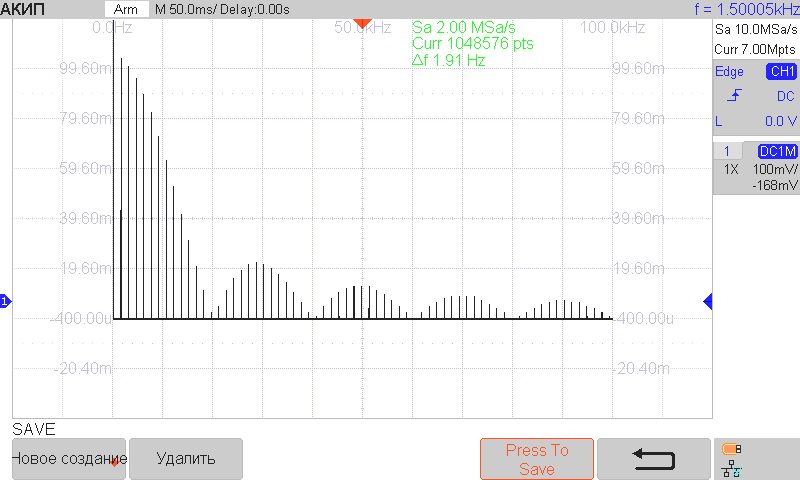
\includegraphics[width=0.5\textwidth]{AKIP0002.png}}}\\
    \end{figure}
\begin{figure}[H]
    \centering
    \subfloat[$\nu_{\text{повт}} = 2$ кГц, $\tau = 50$ мкс]{{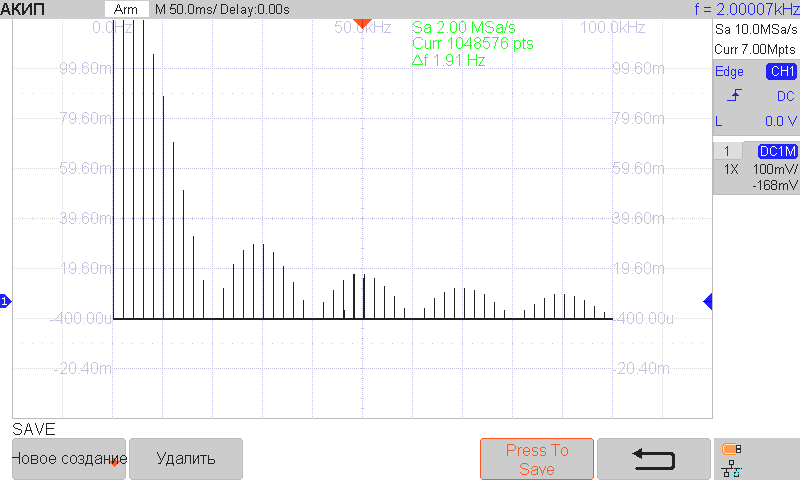
\includegraphics[width=0.5\textwidth]{AKIP0003.png}}}
    \subfloat[$\nu_{\text{повт}} = 2.5$ кГц, $\tau = 50$ мкс]{{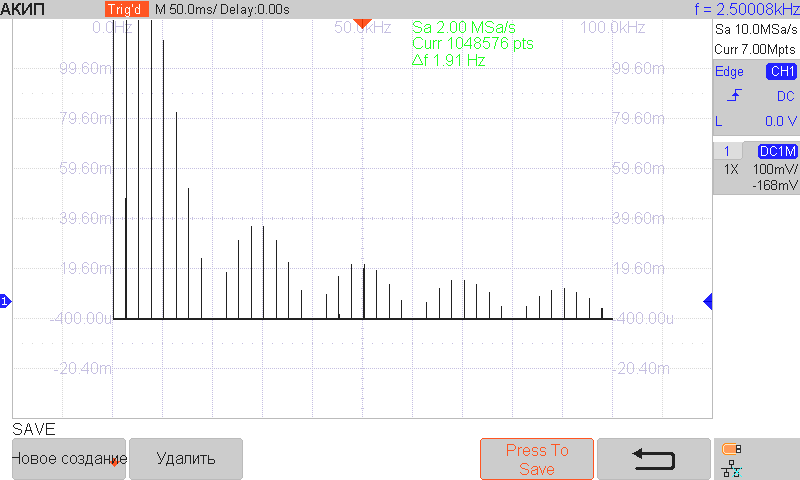
\includegraphics[width=0.5\textwidth]{AKIP0004.png}}}\\
    \end{figure}
\begin{figure}[H]
    \centering
    \subfloat[$\nu_{\text{повт}} = 1$ кГц, $\tau = 60$ мкс]{{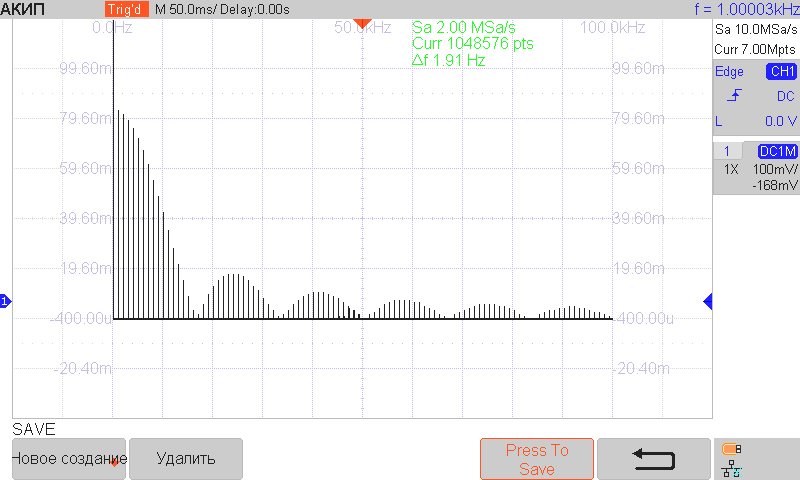
\includegraphics[width=0.5\textwidth]{AKIP0005.png}}}
    \subfloat[$\nu_{\text{повт}} = 1$ кГц, $\tau = 100$ мкс]{{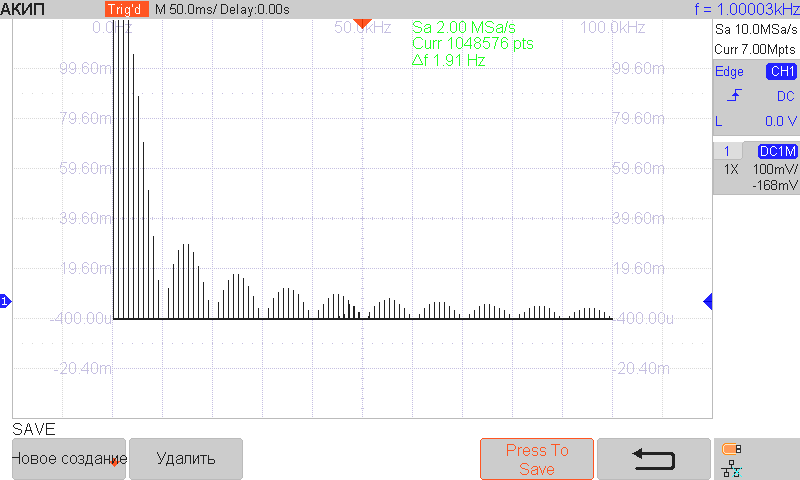
\includegraphics[width=0.5\textwidth]{AKIP0006.png}}}\\
    \end{figure}
\begin{figure}[H]
    \centering
    \subfloat[$\nu_{\text{повт}} = 1$ кГц, $\tau = 150$ мкс]{{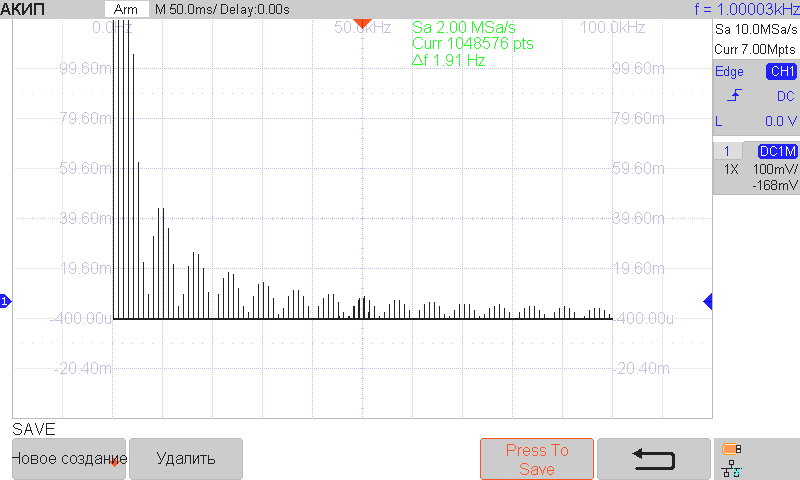
\includegraphics[width=0.5\textwidth]{AKIP0007.png}}}
\end{figure}
\n
Проведя измерения зависимости ширины спектра от $\Delta \nu$, установили связь между $\Delta \nu$ и $\tau$, полученную из формулы $(6)$:
\begin{center}
\begin{tabular}{|c|c|c|c|c|c|c|c|}
\hline
$\tau$, мкс & 50 & 75 & 100 & 125 & 150 & 175 & 200 \\ \hline
$\Delta \nu$, кГц & 19.6 & 13.4 & 9.8 & 8.0 & 6.5 & 5.5 & 4.5 \\ \hline
$1/\tau \cdot 10^3$, с$^{-1}$ & 20 & 13 & 10 & 8 & 7 & 6 & 5 \\ \hline
\end{tabular}
\end{center}
\begin{center}
\fbox{$\Delta \nu \tau = 1,00 \pm 0,02$}
\end{center}
Формула $(6)$ действительно выполняется.

\subsection*{Исследование спектра периодической последовательности цугов}
На экране была получена последовательность цугов с характерными параметрами: $\nu_0 = 50$ кГц, $T = 1$ мс, число периодов в одном импульсе $N = 5$ (длительность импульса $\tau = T/\nu_0 = 100$ мкс).
\begin{figure}[H]
    \centering
    \subfloat[Последовательность цугов]{{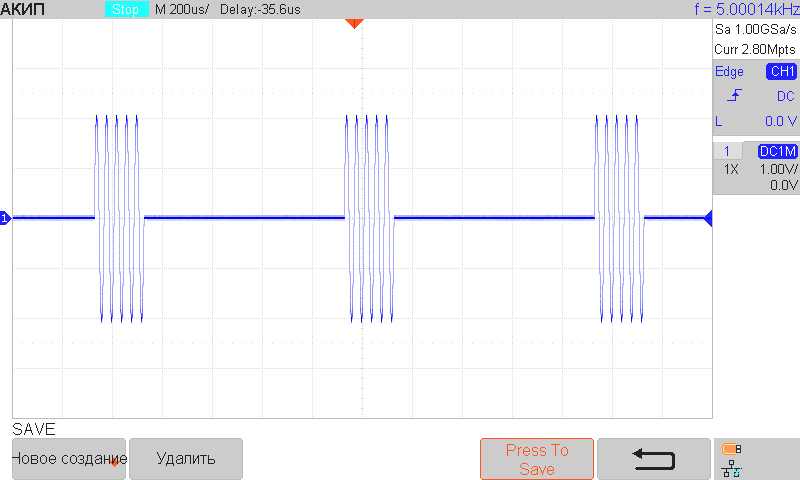
\includegraphics[width=0.5\textwidth]{AKIP0008.png}}}
    \subfloat[Спектр для цугов]{{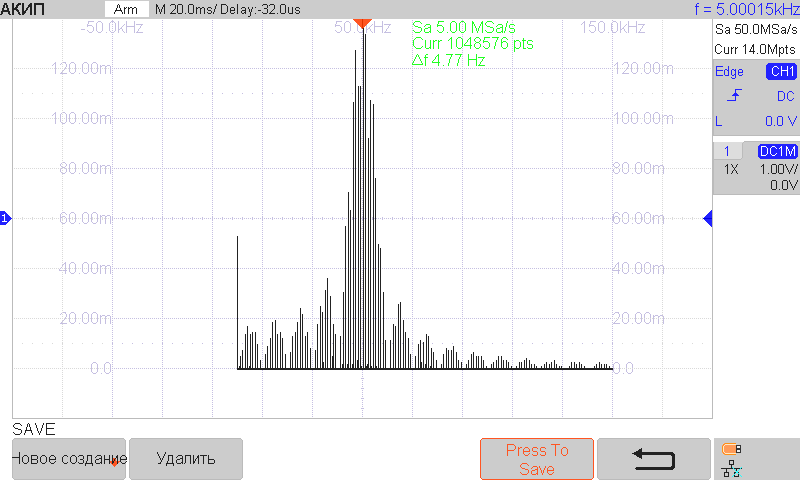
\includegraphics[width=0.5\textwidth]{AKIP0009.png}}}
\end{figure}
\n
Мы изменяли эти параметры по одному и фиксировали результат:
\begin{figure}[H]
    \centering
    \subfloat[$\nu_0 = 50$ кГц, $T = 1$ мс, $N = 10$]{{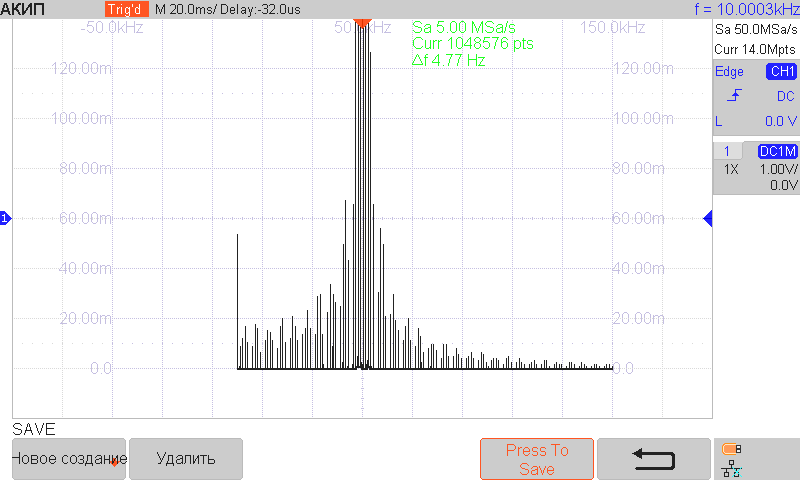
\includegraphics[width=0.5\textwidth]{AKIP0010.png}}}
    \subfloat[$\nu_0 = 50$ кГц, $T = 1$ мс, $N = 15$]{{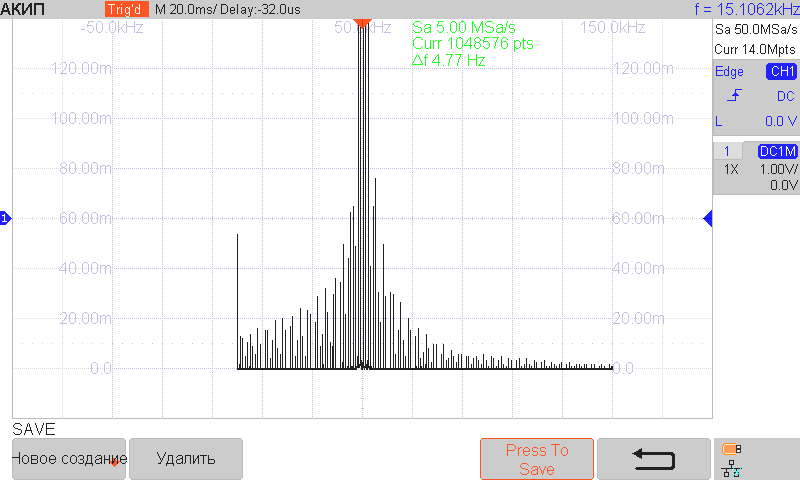
\includegraphics[width=0.5\textwidth]{AKIP0011.png}}}\\
    \end{figure}
    \begin{figure}[H]
    \centering
    \subfloat[$\nu_0 = 50$ кГц, $T = 2.5$ мс, $N = 5$]{{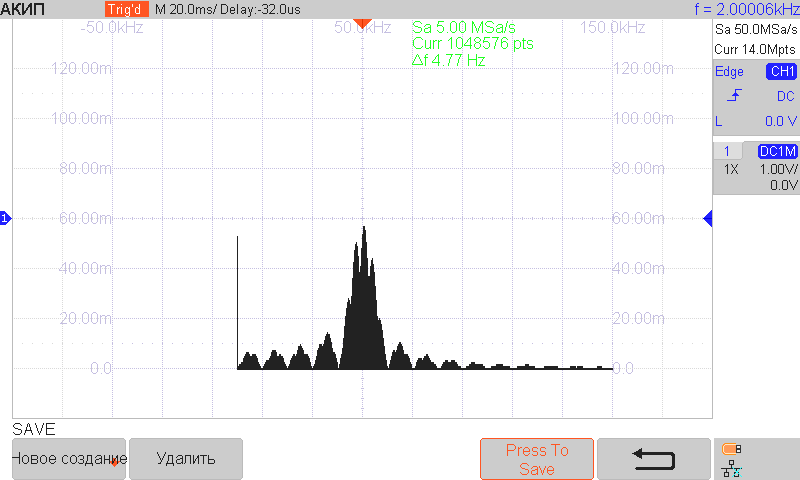
\includegraphics[width=0.5\textwidth]{AKIP0013.png}}}
    \subfloat[$\nu_0 = 50$ кГц, $T = 5$ мс, $N = 5$]{{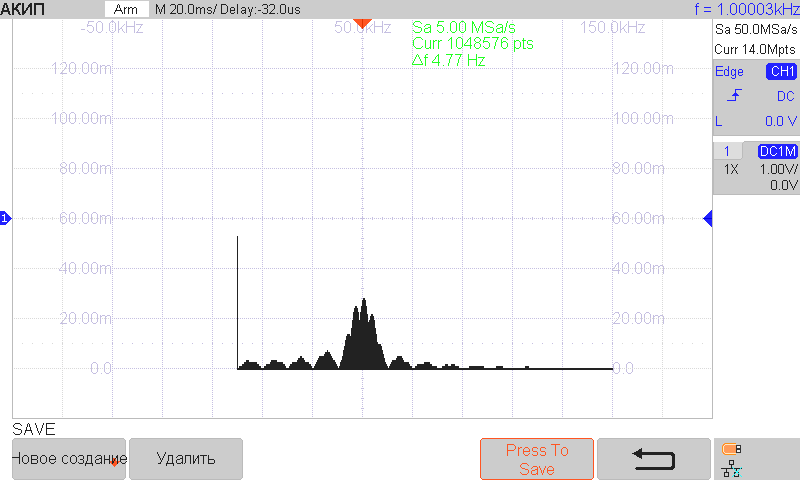
\includegraphics[width=0.5\textwidth]{AKIP0012.png}}}\\
\end{figure}
\begin{figure}[H]
    \centering
    \subfloat[$\nu_0 = 75$ кГц, $T = 1$ мс, $N = 5$]{{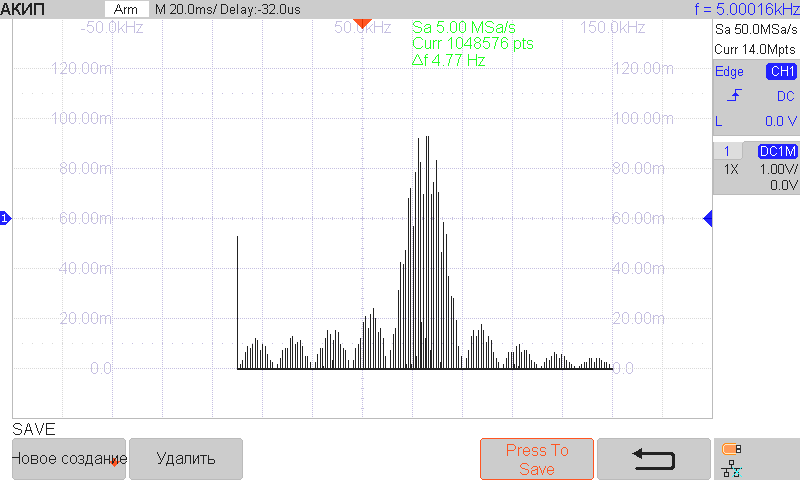
\includegraphics[width=0.5\textwidth]{AKIP0015.png}}}
    \subfloat[$\nu_0 = 100$ кГц, $T = 1$ мс, $N = 5$]{{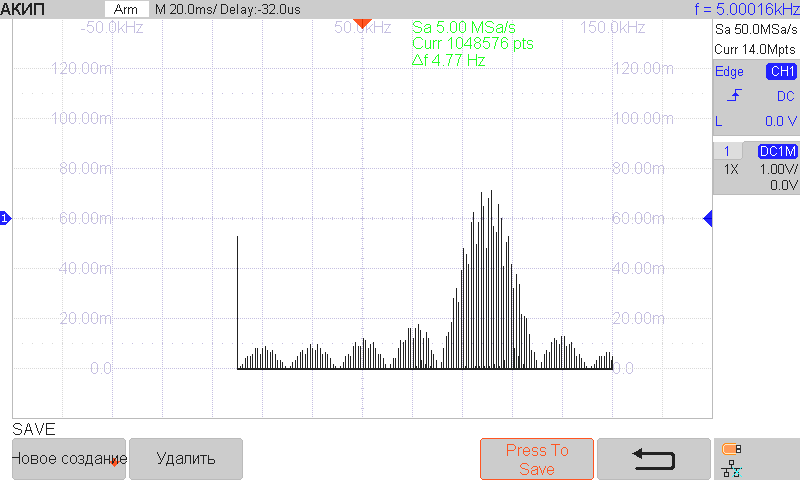
\includegraphics[width=0.5\textwidth]{AKIP0014.png}}}\\
\end{figure}
\n
Далее мы зафиксировали $\nu_0 = 50$ кГц, $N = 5$. Для этих параметров измерили, меняя $T$ ($\nu_{\text{повт}})$, зависимость $\delta \nu$ от $\tau$.
\begin{table}[H]
\centering
\begin{tabular}{|r|r|r|r|r|r|r|}
\hline
$\Delta \nu$, кГц       & 23 & 32 & 35 & 38 & 35 & 45 \\ \hline
$n$                                                   & 42 & 33 & 18 & 13 & 10 &  8 \\ \hline
$\nu_{\text{повт}}$, кГц & 0.5 & 1.0  & 2.0  & 3.0  & 4.0 & 6.0  \\ \hline
\end{tabular}
\end{table}
Итоговое отношение:
\fbox{$\dfrac{\delta \nu}{\nu_{\text{повт}}} = 1,05 \pm 0,08$}
\subsection*{Исследование спектра амплитудно-модулированного сигнала}
На экран выводилась картина амплитудно-модулированного сигнала с характерными параметрами: несущая частота $\nu_0 = 50$ кГц, $\nu_{\text{мод}} = 2$ кГц, глубина модуляции - 50 \% ($m = 0.5$). Картины данного сигнала и его спектра выглядят следующим образом:
\begin{figure}[H]
\centering
 \subfloat[Амплитудно-модулированный сигнал]{{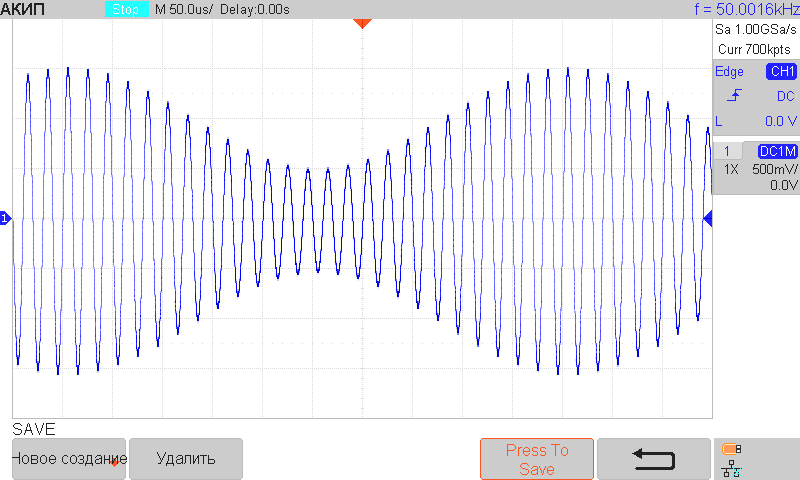
\includegraphics[width = 0.5\textwidth]{AKIP0016.png}}}
    \subfloat[Спектр для $\nu_0 = 50$ кГц, $\nu_{\text{мод}} = 2$ кГц]{{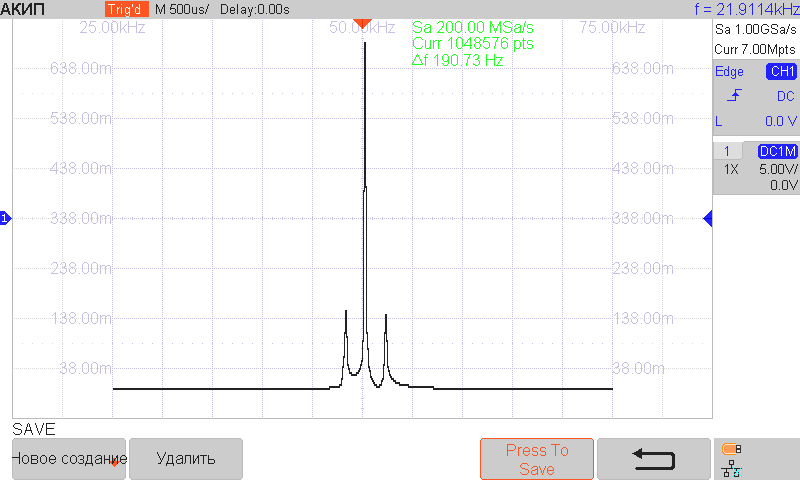
\includegraphics[width=0.5\textwidth]{AKIP0018.png}}}
\end{figure}
\n
Найдем для этого сигнала $A_{max}$ и $A_{min}$ и проверим справедливость формулы $(9)$:
\[A_{max} = 1,52 \text{ В}, \quad A_{min} = 0,48 \text{ В}, \quad m = 0,52\]
\n
Поскольку мы установили глубину модуляции на $0.5$, а из теоретических расчётов получили $0.52$, то видно, что формула $(9)$ верна.
\n\n
Затем мы получили на экране спектр и изменяли параметры сигнала:
\begin{figure}[H]
    \centering
    \subfloat[$\nu_0 = 60$ кГц, $\nu_{\text{мод}} = 2$ кГц]{{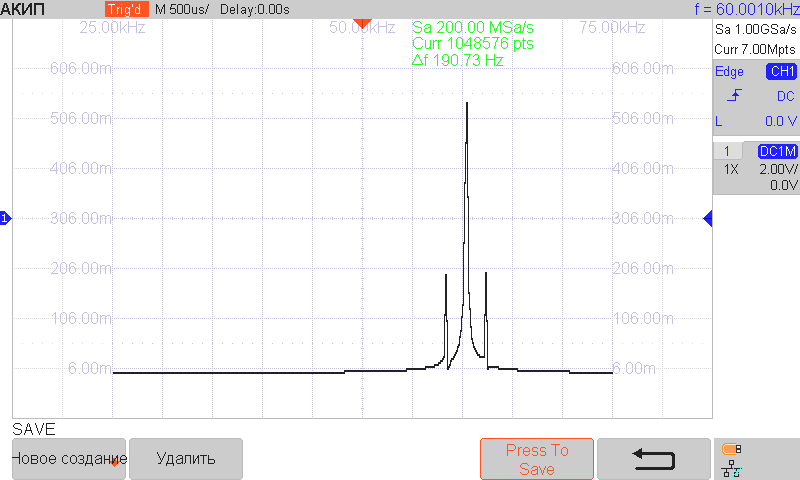
\includegraphics[width=0.5\textwidth]{AKIP0019.png}}}
    \subfloat[$\nu_0 = 70$ кГц, $\nu_{\text{мод}} = 2$ кГц]{{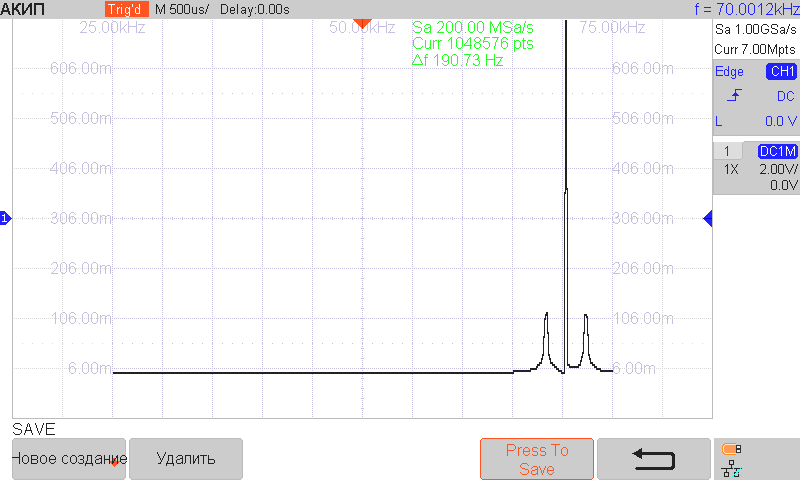
\includegraphics[width=0.5\textwidth]{AKIP0020.png}}}\\
    \end{figure}
    \begin{figure}[H]
    \centering
    \subfloat[$\nu_0 = 50$ кГц, $\nu_{\text{мод}} = 8$ кГц]{{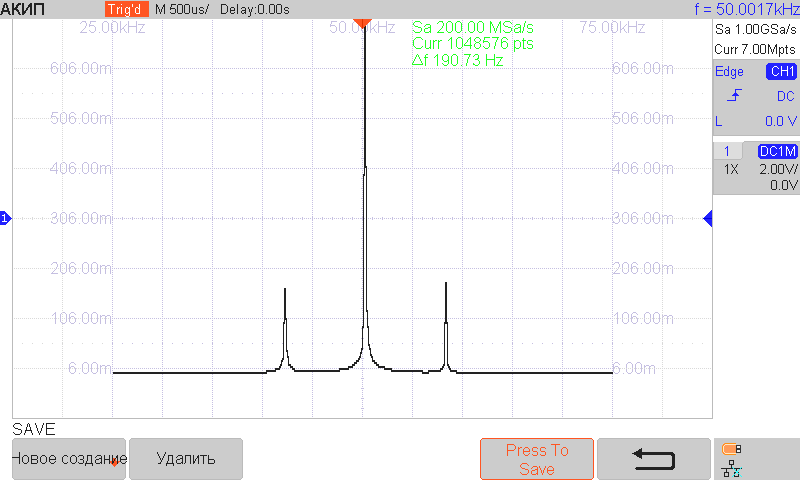
\includegraphics[width=0.5\textwidth]{AKIP0021.png}}}    			\subfloat[$\nu_0 = 50$ кГц, $\nu_{\text{мод}} = 16$ кГц]{{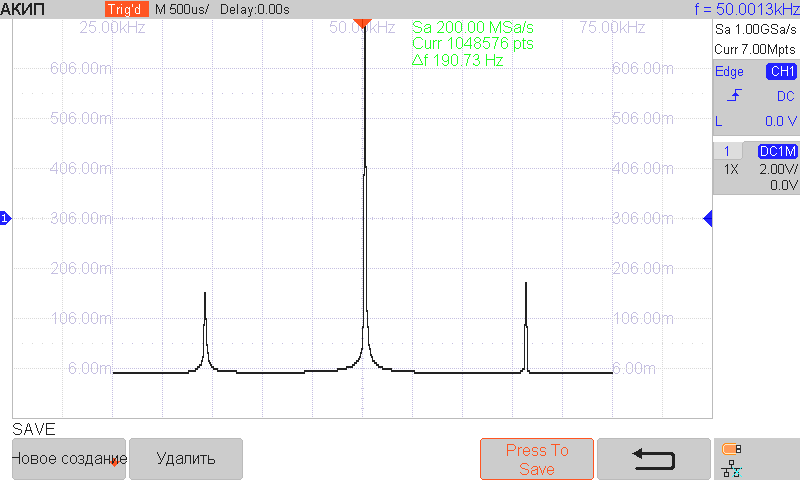
\includegraphics[width=0.5\textwidth]{AKIP0022.png}}}
\end{figure}\n
Из формулы $(10)$ следует, что $a_{\text{осн}} = A_0$, а $a_{\text{бок}} = \dfrac{mA_0}{2}$.
\begin{center}
\begin{tabular}{|c|c|c|c|c|c|}
\hline
$m$, \% & 10 & 25 & 50 & 75 & 100 \\ \hline
$a_{\text{бок}}$, мВ & 360 & 820 & 1660 & 2320 & 3260 \\ \hline
$a_{\text{осн}}$, мВ & 6240 & 6240 & 6240 & 6240 & 6240 \\ \hline
$a_{\text{бок}}/a_{\text{осн}}$ & 0.06 & 0.13 & 0.27 & 0.37 & 0.52 \\ \hline
$a_{\text{бок}}/a_{\text{осн}} \cdot m$, \% & 57.7 & 52.6 & 53.2 & 49.6 & 52.2 \\ \hline
\multicolumn{6}{|c|}{$a_{\text{бок}}/a_{\text{осн}} \cdot m = (53,1 \pm 1,3)$\%} \\ \hline
\end{tabular}
\end{center}
Из $(10)$ имеем $\dfrac{a_{\text{бок}}}{a_{\text{осн}}} \cdot m = 0.5$, что с высокой точностью повторяет наш результат.
\n
\section*{Заключение}
Исследования зависимости ширины спектра периодической последовательности прямоугольных импульсов от длительности отдельного импульса в первой части работы полностью совпали с теоретическими рассчетами. По наклону графика из этой части можно убедиться в соотношении неопределенностей ($\Delta \nu \Delta t \simeq 1$).
\n\n
Исследования зависимости расстояния между ближайшими спектральными компонентами от частоты повторения цугов дали схожие результаты.
\n\n
В последней части коэффициенты, получаемые в результате исследования зависимости отношения амплитуд спектральных линий синусоидального сигнала, модулированного низкочастотными гармоническими колебаниями, от коэффициента модуляции полностью совпали с теоретически рассчитаными.


\include{matlab}

\end{document}
